\subsection{A low-resource language: Bengali clickbait}\label{sec:bangla}
\paragraph{Replication and duplicates}
On the official BanglaBait split, character 3--5-gram logistic regression reaches a clickbait-class F1 of \BBrelFone{} (Figure~\ref{fig:bengali}a), within two points of the 66.28 reported for the same model by \citet{mahtab2023banglabait}, and a linear SVM reaches \BBrelSVMFone{}. Removing the near-duplicates found by MinHash from the official splits lowers the same model to \BBdedFone{} (AUC \BBrelAUC{}$\to$\BBdedAUC{}): even after the original authors' Levenshtein filter, duplicated titles inflate the benchmark. Over five random re-splits of the deduplicated corpus the model reaches AUC \BBseedAUC{} $\pm$ \BBseedAUCsd{}.

\paragraph{Publisher identity}
The \BBnPub{} publishers with at least 100 articles have clickbait rates from \BBrateMin{} to \BBrateMax{}, so publisher identity alone predicts the label with AUC \BBgroupAUC{} (Section~\ref{sec:shortcuts}). Leave-one-publisher-out evaluation nevertheless costs little: across \BBlosoN{} held-out publishers (the smallest ones pooled), mean AUC is \BBlosoAUC{} (range \BBlosoMin--\BBlosoMax), close to the random-split value. Bengali clickbait detection survives a change of source that English veracity detection does not. One reading is that this is a construct effect rather than a language effect. Clickbait \emph{is} a property of a headline's style, so a style-sensitive detector can learn the construct itself, whereas for veracity, style is only a correlate of the label that changes from corpus to corpus. The comparison is not fully controlled, though: BanglaBait was labelled by annotators reading each headline, while the English veracity labels come from fact-checks or from the outlet an article was taken from, so how the labels were made differs as well as what they mean.

\paragraph{Across languages}
A translate-test probe uses BanglaBait's machine-translated English titles. A detector trained on English clickbait headlines \citep{chakraborty2016clickbait} ranks translated Bengali titles with AUC \XlENtoBB{}, against \XlBBEN{} for a detector trained on the translated titles themselves and \XlBN{} for one trained on the original Bengali; translation costs about \XlTransCost{} AUC and most of the in-language ranking ability carries over. In the other direction, the translated-Bengali detector reaches \XlBBtoEN{} on English headlines (in-domain \XlEN). Clickbait carries over across languages much better than veracity carries over across English corpora, although translation and the change of collection still cost about 0.1 AUC (\XlENtoBB{} against \XlBN{} in-language).

\begin{figure}[t]
\centering
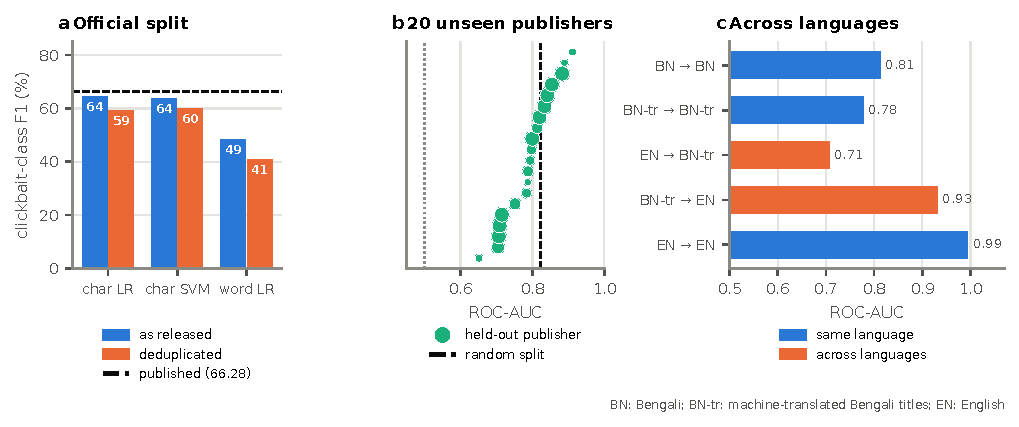
\includegraphics[width=\linewidth]{fig_bengali}
\caption{Bengali clickbait. (a)~Clickbait-class F1 on the official BanglaBait split, as released and after removing near-duplicates, against the published value for character LR \citep{mahtab2023banglabait}. (b)~ROC-AUC on each held-out publisher (dot size: number of articles) against the random-split value. (c)~Translate-test: training and test corpora in Bengali (BN), machine-translated Bengali titles (BN-tr) or English clickbait headlines (EN).}\label{fig:bengali}
\end{figure}
